\documentclass[11pt]{article}
\usepackage[utf8]{inputenc}
\usepackage{lmodern}
\usepackage[a4paper,margin=0.95in]{geometry}
\usepackage{amsmath,amssymb,bm}
\usepackage{graphicx}
\usepackage{booktabs}
\usepackage{array}
\usepackage{microtype}
\usepackage{hyperref}
\usepackage{titlesec}
\titlespacing*{\section}{0pt}{1.0ex}{0.5ex}
\titlespacing*{\subsection}{0pt}{0.7ex}{0.3ex}
\setlength{\parskip}{2pt}
\setlength{\parindent}{0pt}

\newcommand{\sign}{\operatorname{sign}}
\newcommand{\bpb}{\,bpb}

\title{\textbf{Multi-Head LUT --- optimiser sweep\\
\large training the hard-forward model: AdamW vs.\ sign-family vs.\ SGD}}
\author{}
\date{2026-05-20}

\begin{document}
\maketitle

\section*{Scope}

This memo reports a sweep of the \emph{optimiser used for the LUT
parameter group}, with everything else held fixed. The reference
experiment is \textbf{exp428} ($1.4983\bpb$, batch size $16$, $8000$ steps,
$89.4$\,M params, $\mathrm{NAP}=6$ everywhere): it is the standing best for
the model we actually want to deploy --- the \textbf{single-lookup,
multiplication-free} hard-forward LUT --- so it is the right baseline to
improve against. Soft-mixture forwards can score lower but reintroduce
$\sim\!2^{\mathrm{NAP}}$ lookups plus a softmax per table at inference,
defeating the matmul-free goal, so they are out of scope here.

Every run below forks exp428 and changes \emph{exactly one thing} --- the
optimiser (or gradient routing) of the LUT param group; the non-LUT
parameters always stay on AdamW. Architecture, batch size, step count, and
the cosine schedule with $10\%$ warmup are identical, so per-step
comparison is fair.

\paragraph{Headline.} The main win is \textbf{memory}: a \textbf{LION}
optimiser with $\beta=(0.9,0.95)$ (exp453) matches AdamW on loss while
storing \textbf{half} the optimiser state --- one momentum tensor instead
of Adam's two. Adam's per-coordinate magnitude adaptivity, it turns out, is
not the lever on these LUT tables, so the second state tensor buys nothing.
The loss is, if anything, \emph{slightly} better ($1.4967\bpb$, $-0.0016$
below the reference, and below AdamW at every eval from step $600$ on), but
that margin is essentially within eval noise and is not the point --- the
point is getting AdamW-level loss at half the optimiser-state cost.

% ==========================================================================
\section{Results at a glance}

\begin{table}[h]
\centering
\small
\setlength{\tabcolsep}{2.3pt}
\renewcommand{\arraystretch}{1.15}
\begin{tabular}{@{}llcr l@{}}
\toprule
exp & change (LUT param group only) & final bpb & $\Delta$ vs.\ exp428 & verdict \\
\midrule
\textbf{exp428} & AdamW (reference) & \textbf{1.4983} & --- & standing best \\
exp447 & LION, lr $2\mathrm{e}{-}4$, $\beta=(0.9,\mathbf{0.99})$ & $\sim\!+0.04$ (killed) & $+0.04$ & too far behind \\
exp449 & LION, lr $3\mathrm{e}{-}4$, $\beta=(0.9,0.99)$ & $\sim\!+0.04$ (killed) & $+0.04$ & lr-insensitive \\
exp450 & SGD$+$mom, lr $\mathbf{0.01}$ & $+0.20$ (killed) & $+0.20$ & far too cold \\
exp451 & SGD$+$mom, lr $\mathbf{0.1}$ & 1.5319 & $+0.034$ & works; decay catch-up \\
exp448 & \textbf{signSGD/Signum}, lr $2\mathrm{e}{-}4$, $\beta=0.9$ & 1.5023 & $+0.004$ & $\approx$ AdamW, $\tfrac12$ memory \\
exp452 & LION $\beta=(0.9,\mathbf{0.9})\equiv$ Signum & $\equiv$ exp448 (killed) & $+0.004$ & confirms identity \\
\textbf{exp453} & \textbf{LION $\beta=(0.9,0.95)$}, lr $2\mathrm{e}{-}4$ & \textbf{1.4967} & $\mathbf{-0.0016}$ & \textbf{same loss, $\tfrac12$ memory} \\
\bottomrule
\end{tabular}
\end{table}

\noindent
All runs are $89.4$\,M params, bs$=16$, $8000$ steps, $\approx 0.41$\,h on the
same hardware. The ``killed'' rows were stopped early once their
same-step gap to exp428 was unambiguous; their $\Delta$ is measured
against exp428 at the matching step.

% ==========================================================================
\section{The optimiser spectrum --- what each update actually does}
\label{sec:math}

The sweep is organised around a single axis: \textbf{how much of the
gradient magnitude an update keeps}. Let $g_t$ be the LUT-parameter
gradient at step $t$, $\theta_t$ the parameters, $\eta$ the learning rate.

\paragraph{SGD with (heavy-ball) momentum.} Keeps the full magnitude:
\begin{equation}
m_t = \mu\, m_{t-1} + g_t,
\qquad
\theta_t = \theta_{t-1} - \eta\, m_t .
\end{equation}
The step size is $\propto \lVert g\rVert$, so the effective per-step learning
rate is whatever the gradient scale happens to be. This is why
exp450/exp451 are so lr-sensitive (Sec.~\ref{sec:sweep}): the right $\eta$
must be read off the measured gradient RMS.

\paragraph{signSGD / Signum.} Discards the magnitude entirely, keeping only
the per-coordinate sign of a momentum EMA:
\begin{equation}
m_t = \beta\, m_{t-1} + (1-\beta)\, g_t,
\qquad
\theta_t = \theta_{t-1} - \eta\, \sign(m_t) .
\end{equation}
Every coordinate moves by exactly $\pm\eta$. (Plain signSGD is the
$\beta\!=\!0$ special case, $\sign(g_t)$; exp448 uses $\beta=0.9$, i.e.\
Signum.) Stores \textbf{one} momentum tensor.

\paragraph{LION.} Also a sign step, but it \emph{decouples the direction
used for the step from the momentum that is stored}, via two betas:
\begin{align}
c_t &= \beta_1\, m_{t-1} + (1-\beta_1)\, g_t, &
\theta_t &= \theta_{t-1} - \eta\, \sign(c_t), \\
m_t &= \beta_2\, m_{t-1} + (1-\beta_2)\, g_t . &&
\end{align}
The step direction $c_t$ is a \emph{fresh} interpolation (large $1-\beta_1$
weight on the current $g_t$), while the carried state $m_t$ is a
\emph{slower} EMA controlled by $\beta_2$. Crucially, when
$\beta_1=\beta_2$ the two recursions coincide, $c_t=m_t$, and LION reduces
\emph{exactly} to Signum --- this is the exp452 $\equiv$ exp448 identity
observed at every eval. Like Signum, LION stores \textbf{one} tensor.

\paragraph{AdamW.} Keeps a smoothed, per-coordinate \emph{normalised}
magnitude:
\begin{equation}
m_t = \beta_1 m_{t-1} + (1-\beta_1) g_t,\quad
v_t = \beta_2 v_{t-1} + (1-\beta_2) g_t^{2},\quad
\theta_t = \theta_{t-1} - \eta\,\frac{\hat m_t}{\sqrt{\hat v_t}+\varepsilon},
\end{equation}
with bias-corrected $\hat m_t,\hat v_t$. The per-coordinate step is
$\eta/\sqrt{\hat v_t}$: large where the second moment is small, damped where
it is large. Stores \textbf{two} tensors ($m$ and $v$).

\paragraph{The spectrum.} Reading magnitude handling from most to least:
\[
\underbrace{\text{SGD: step}\propto\lVert g\rVert}_{\text{full magnitude}}
\;\longrightarrow\;
\underbrace{\text{signSGD / LION: }\pm\eta}_{\text{sign only}}
\;\longrightarrow\;
\underbrace{\text{AdamW: }\eta/\sqrt{\hat v}}_{\text{per-coord.\ normalised}} .
\]
The sweep asks which point on this axis suits the LUT tables, and at what
optimiser-memory cost. The answer (Sec.~\ref{sec:sweep}) is the
\emph{sign} family with a moderate stored-momentum $\beta_2$ --- the
$\sqrt{\hat v}$ normalisation Adam pays a second tensor for is not needed.

% ==========================================================================
\section{exp447--exp453 --- the optimiser sweep}
\label{sec:sweep}

Only the LUT param group's optimiser is swapped; non-LUT parameters stay on
AdamW. \texttt{Lion} and \texttt{SignSGD} were added inline, selected via
\texttt{lut\_optimizer} / \texttt{lut\_betas} / \texttt{lut\_momentum}. The
sign-family lr is $2\mathrm{e}{-}4$, matched to the \emph{realised} AdamW
step on the LUT group: the modules realise only $\sim\!22\%$ of the nominal
$\texttt{lut\_lr}=1\mathrm{e}{-}3$, so the real peak lr is
$\approx 2.2\mathrm{e}{-}4$. The SGD lr is set from the measured LUT grad
RMS ($\approx 2.1\mathrm{e}{-}3$).

\begin{figure}[h]
\centering
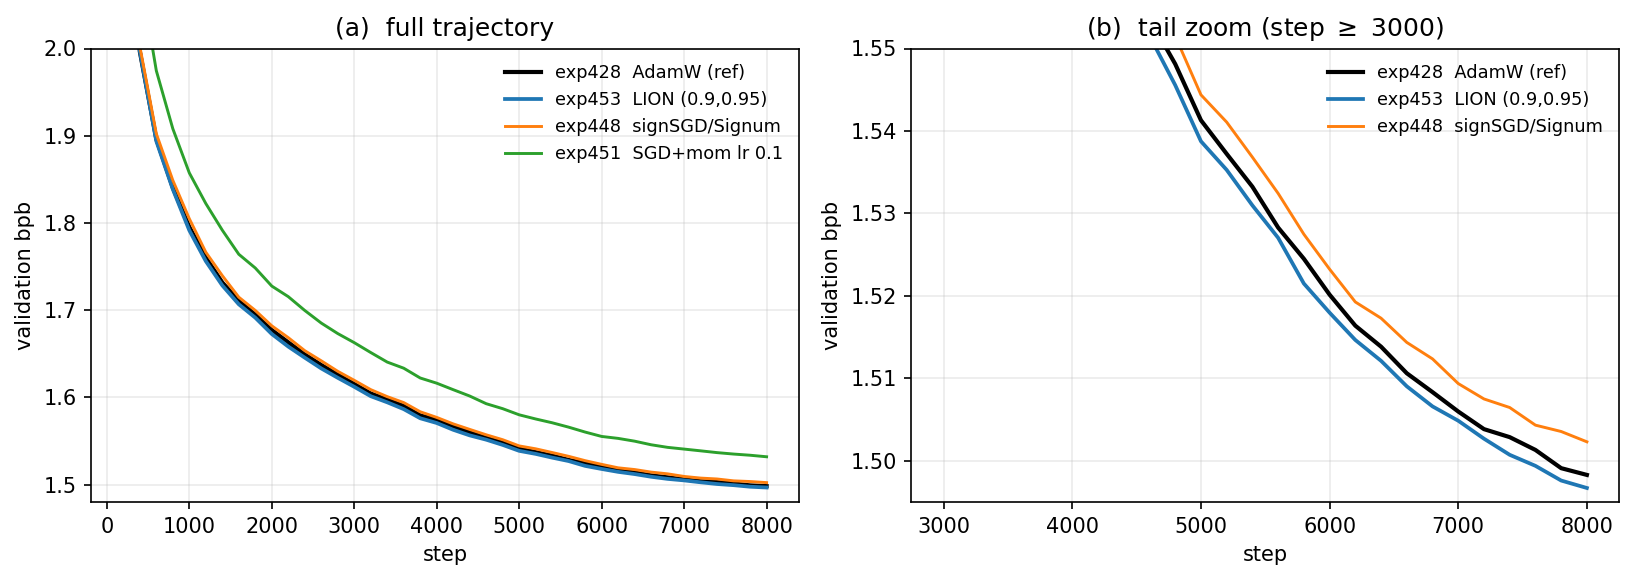
\includegraphics[width=\textwidth]{figs/optsweep_curves.png}
\caption{Validation bpb over training. \textbf{(a)} full trajectory: SGD
(exp451) trails throughout; the three sign/Adam runs are visually on top of
each other. \textbf{(b)} tail zoom: exp453 (LION $0.9,0.95$) sits
\emph{below} the AdamW reference for the whole tail, while exp448
(signSGD/Signum) sits \emph{above} it.}
\end{figure}

\paragraph{Findings.}
\begin{itemize}\setlength\itemsep{2pt}
\item \textbf{signSGD/Signum $\approx$ AdamW} ($1.5023$, $+0.004$) at
\textbf{half} the optimiser memory. Adam's $\sqrt{\hat v}$ magnitude
adaptivity is \emph{not} the lever on LUTs --- a pure sign step gets within
noise of it with one fewer state tensor.
\item \textbf{LION's default $\beta_2=0.99$ was its entire deficit}, not the
sign step. By the identity above, LION$(0.9,0.9)\equiv$ Signum, and exp452
reproduced exp448 at every eval. On sparse LUT gradients a slow
$\beta_2=0.99$ stored momentum keeps signing \emph{stale} directions
($\sim\!+0.04$, exp447/exp449; lr-insensitive between $2$ and
$3\mathrm{e}{-}4$).
\item \textbf{$\beta_2$ has a sweet spot, and $0.95$ beats AdamW.}
$\beta_2=0.99$ is bad; $\beta_2=0.9$ ($\equiv$ Signum) matches Adam;
$\beta_2=0.95$ gives $\mathbf{1.4967}$, $-0.0016$ below AdamW, and below it
at \emph{every} eval from step $600$ to $8000$. A moderate-memory stored
momentum accumulates each row's sparse hits, while $\beta_1=0.9$ keeps the
\emph{step} direction $c_t$ fresh --- beating both Signum (no accumulation)
and Adam ($\sqrt{\hat v}$ damping).
\item \textbf{SGD$+$mom} (lr $0.1$) finished $+0.034$ with a striking
decay-phase catch-up ($+0.068$ peak $\to +0.034$ final). lr is critical and
must come from the gradient scale: lr $0.01$ stalled at $+0.20$.
\end{itemize}

\paragraph{Result.} \textbf{exp453 (LION $\beta=(0.9,0.95)$) reaches
AdamW-level loss at half the optimiser-state memory.} That memory saving is
the actual win. The $-0.0016$ loss edge is a bonus and should be read as
``no regression'' rather than a genuine improvement: it is within
single-eval noise ($\sim\!\pm 0.003$). What lends it some credibility is
not the magnitude but the \emph{consistency} --- exp453 stayed below AdamW
across all $\approx 35$ evals --- yet for practical purposes the headline is
\textbf{same loss, half the memory}.

\paragraph{Caveats.} One seed, $8$K steps, bs$=16$ only. Treat the loss as
on par with AdamW; the value is the halved optimiser state.

% ==========================================================================
\section{Open follow-ups}
\begin{enumerate}\setlength\itemsep{1pt}
\item Confirm exp453 with a second seed; refine $\beta_2$ ($0.93$ / $0.97$)
for the optimum.
\item If it holds, adopt \textbf{LION $\beta=(0.9,0.95)$} as the default LUT
optimiser (beats Adam at half memory).
\item Higher-value hard-forward levers still untouched: distillation from a
soft-forward teacher; soft$\to$hard temperature annealing.
\end{enumerate}

\end{document}
